
\chapter{Модельный порыв}

\section{Введение} 


В круглой трубе течение Пуазейля устойчиво к малым возмущениям. Для выхода на турбулентное решение, стартуя с возмущенного течения Пуазейля, амплитуда возмущения должна быть достаточно велика. Кроме амплитуды возмущнеия имеет значения также его форма. В частности, любые осесимметричные возмущения течения Пуазейля затухают. Для начального возмущения фиксированной формы можно определить такое значение амплитуды, что решение в процессе эволюции будет оставаться на сепаратрисе, разделяющей в фазовом пространстве области притяжения ламинарного и турбулентного решений. Это решение неустойчиво и при численном интегрировании рано или поздно сваливается в ту или иную сторону --- либо выходит на турбулентный режим, либо возвращается к течению Пуазейля. Тем не менее, варьируя начальную амплитуду возмущения, можно проследить поведение балансирующего на сепаратрисе решения на значительном промежутке времени. Как показано в \cite{Skufca2006}, предельное решение, к которому стремится решение на сепаратрисе, сохраняет некоторые черты турбулентного решения, но при этом как правило обладает более простым поведением во времени. В \cite{Avila2013} обнаружено, что при наложении дополнительных ограничений симметрии предельное решение на сепаратрисе при $Re\sim2000$ качественно близко к турбулентному порыву, но оказывается при этом условно-периодическим по времени, а именно, периодическим в подходящей подвижной системе отсчета. Простота поведения предельного решения на сепаратрисе позволяет провести его исчерпывающее исследование, что на наш взгляд может быть небесполезным для понимания  механизма образования и самоподдержания турбулентных порывов. Мы будем называть решение на сепаратрисе модельным порывом. Основные результаты, приведенные в этом разделе, опубликованы в работах автора \cite{MZG2015, Kazan2015, MZG2017}. 

\section{Поиск решения на сепаратрисе}

Следуя \cite{Avila2013}, решение уравнений Навье--Стокса ищется с дополнительными ограничениями диаметральной симметричности и $\pi$-периодичности поля скорости $\v = (v_x, v_r, v_\theta)$ в угловом направлении:
\begin{equation}\label{sym_eq}
(u_x,u_r)(x,r,-\theta,t)=(u_x,u_r)(x,r,\theta,t),\ \ u_\theta(x,r,-\theta,t)=-u_\theta(x,r,\theta,t)
\end{equation}
\begin{equation}\label{per_eq}
(u_x,u_r,u_\theta)(x,r,\theta+\pi,t) = (u_x,u_r,u_\theta)(x,r,\theta,t)
\end{equation}
Здесь $(x, r, \theta)$ --- цилиндрические координаты. Наложение ограничений \eqref{sym_eq}, \eqref{per_eq} упрощает поведение решения в пространстве, делает его более определенным, но важно, что оно остается решением исходной системы. Турбулентные порывы, рассчитанные при $Re=2000$ с учетом и без учета условий \eqref{sym_eq}, \eqref{per_eq} изображены на фиг.~\ref{3D_img} (представлены области пониженной и повышенной на $0.1$ скорости относительно течения Пуазейля). В обоих случаях порыв имеет центральное ядро с пониженной скоростью и систему вытянутых вдоль стенки трубы, чередующихся в угловом направлении полос замедления и ускорения. На симметричном порыве полосы гораздо более структурированы. Их угловое положение не меняется в процессе эволюции: угловые области $\theta=k\pi/2,\ k=0-3$, где в силу \eqref{sym_eq}, \eqref{per_eq} угловая компонента скорости тождественно равна нулю, заняты полосами ускорения, промежуточные области $\theta=\pi/4+k\pi/2$ --- полосами замедления. На порыве без условий симметрии наблюдаются значительные по амплитуде случайные по пространственному расположению флуктуации, разрывающие сплошность полосчатых структур. На симметричном порыве тоже заметна флуктуирующая компонента, которая в этом случае выглядит гораздо более регулярной. Отметим, что несмотря на заметную пространственную регулярность, временн\'{о}е поведение симметричного порыва остается хаотичным.


\begin{figure}[h]
\center{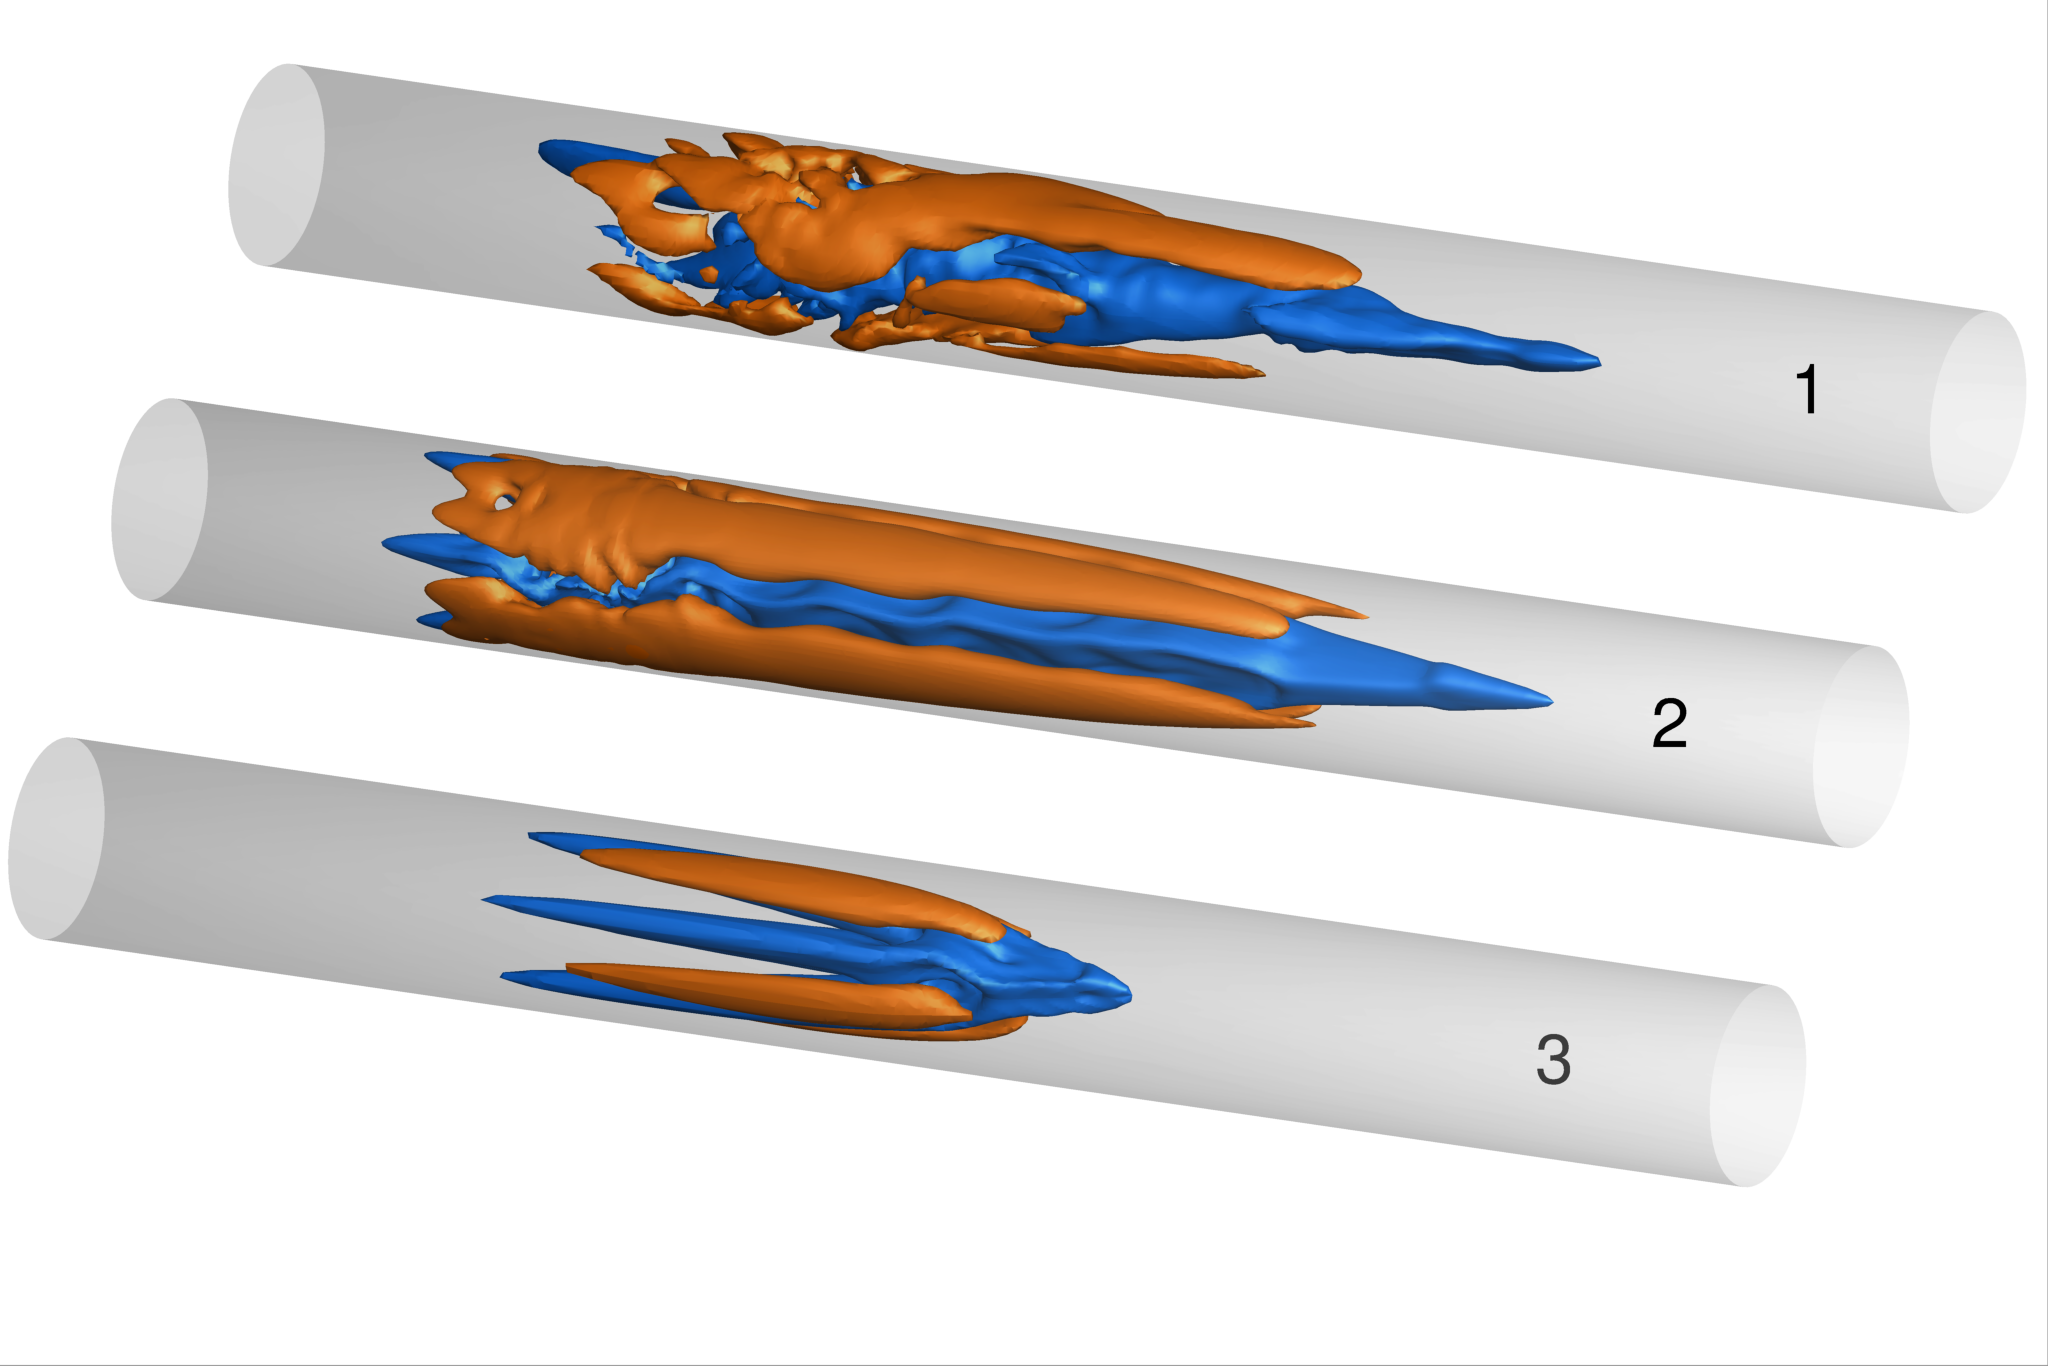
\includegraphics[width=1\linewidth]{3D_cmp.png}}
\caption{Визуализация численных расчетов турбулентных порывов: 1 --- Re = 2000; 2 --- Re = 2000 с учетом \eqref{sym_eq}, \eqref{per_eq}; 3 --- решение на сепаратрисе, Re = 2200. Темным и светлым тоном выделены поверхности скорости –0.1 и + 0.1 относительно скорости течения Пуазейля. Направление потока слева направо.}
\label{3D_img}
\end{figure}

Предельное решение на сепаратрисе рассчитывалось при $Re=2200$. С учетом условий \eqref{sym_eq}, \eqref{per_eq} расчет проводился для четверти объема трубы $0\leqslant\theta\leqslant\pi/2$. Решение на сепаратрисе было найдено на трех сетках. Исходная сетка построена в расчетной области длиной $L_x = 80$ и имеет $512 \times 32 \times  32$ ячеек. Для того, чтобы продемонстрировать, что решение не зависит от длины расчетной области, было также найдено решение при вдвое большем значении $L_x = 160$ на сетке с вдвое большим числом узлов в продольном направлении $1024 \times 32 \times 32$. Для того, чтобы показать сеточную сходимость, решение также было найдено на третьей сетке при исходном значении $L_x=80$ с вдвое большим пространственным разрешением $1024 \times 64 \times 64$. Решения, полученные на каждой из сеток, качественно совпадают и близки количественно, что подтверждает физический характер решения. Решение не зависит от численного метода, так как в работах других авторов решение было найдено другими численнымим метода, в частности спектральным, и наблдается хорошее сходноство характеристик решения. 

Предварительно найденное турбулентное решение $\u_{turb}(\x,t)$ используется в итерационной процедуре отыскания предельного решения на сепаратрисе. Задача решается с начальным условием
\begin{equation*}\label{init}
  \u(\x,t=0) = \u_{Pois}(\x)+\alpha(\u_{turb}(\x,t=t_0) - \u_{Pois}(\x))
\end{equation*}
Здесь $\u_{Pois}=(1-r^2,0,0)$ --- течение Пуазейля, $t_0$ --- некоторый фиксированный момент времени, $\alpha\in[0,1]$ --- скалярный параметр. Значение $\alpha=0$ соответствует нулевому возмущению, и решением при $t>0$ остается течение Пуазейля. Выбирая $\alpha=1$, мы уже в начальный момент времени попадаем на турбулентный режим и остаемся на нем при $t>0$. При промежуточных значениях $\alpha$ происходит стремление решения либо к одному, либо к другому режиму. Применяя метод деления пополам, мы постепенно отыскиваем то значение $\alpha$, при котором решение эволюционирует на сепаратрисе, разделяющей области притяжения двух режимов течения. На фиг.~\ref{bisection_pic} представлены графики $A(t)$ --- среднеквадратичного по всему объему отклонения поля скорости от течения Пуазейля для нескольких значений $\alpha$, демонстрирующие сходимость итерационного процесса. Уточняя значение $\alpha$, мы продлеваем длительность балансирования решения на сепаратрисе.

\begin{figure}[h]
\center{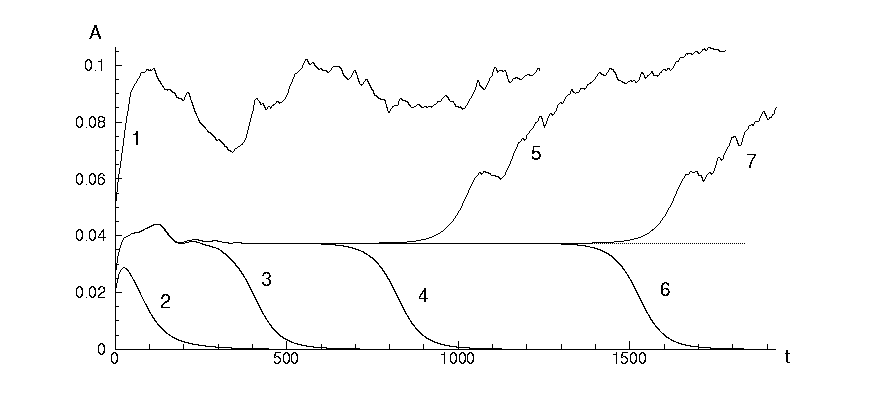
\includegraphics[width=1\linewidth]{bisection.png}}
\caption{Итерационный процесс построения решения на сепаратрисе. 1--7 --- эволюция среднеквадратичной амплитуды возмущений $A(t)$ при уточнении начального
значения.}
\label{bisection_pic}
\end{figure}

В согласии с результатами \cite{Avila2013}, решение на сепаратрисе при $Re=2200$ постепенно выходит на условно периодический режим. Это решение, как и турбулентный порыв, имеет форму локализованой в пространстве структуры, которая сносится вниз по потоку с постоянной скоростью. В подвижной системе отсчета поле скорости в каждой точке испытывает периодические колебания. Для скорости сноса и периода колебаний получены значения $C_f=0.69$ и $T=60$ (в \cite{Avila2013} сообщается о $C_f=0.76$ и $T=60$). Сравнение предельного решения на сепаратрисе с турбулентным порывом, представленное на фиг.~\ref{3D_img}, показывает качественное согласие этих решений. Во всех структурах имеются протяженные области ускоренного и замедленного движения, концентрирующиеся в пристенной области трубы. Сохраняется и основная качественная особенность порыва --- медленное понижение осевой скорости на переднем фронте и более резкое восстановление на заднем. Скорость на оси трубы изобрадена на фиг.~\ref{ucl_cmp_img}. 

\begin{figure}[h]
\center{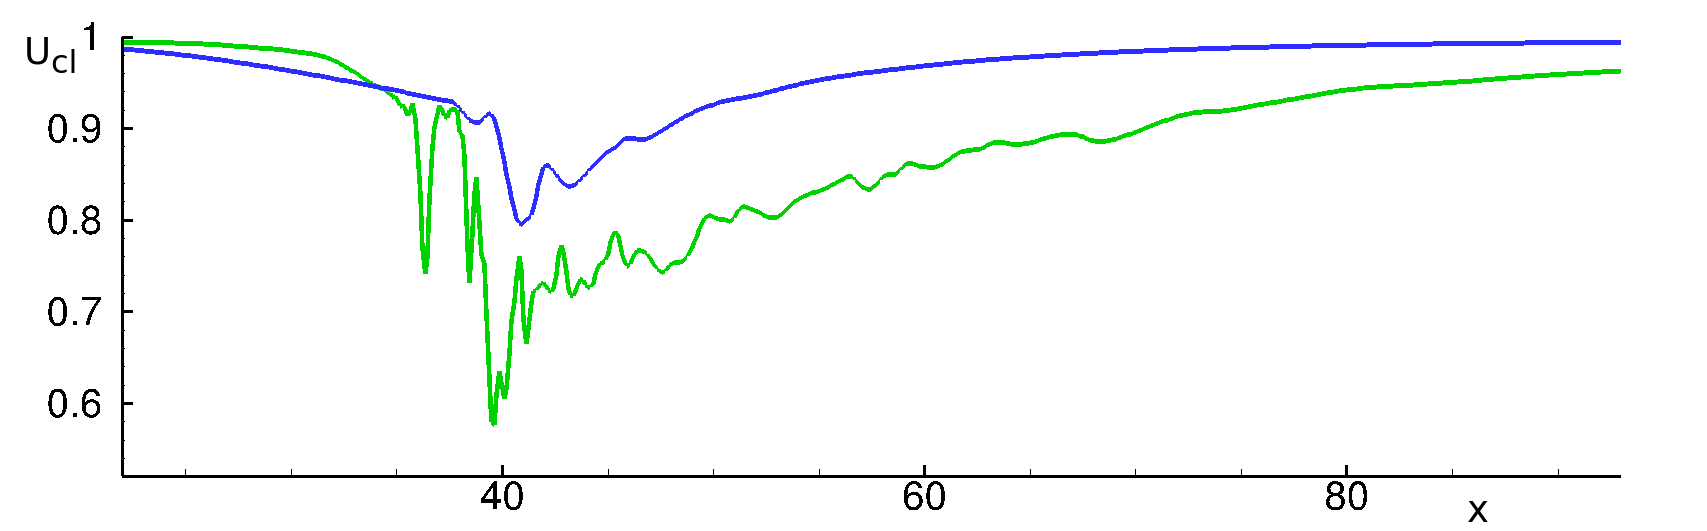
\includegraphics[width=1\linewidth]{ucl_cmp.png}}
\caption{Сравнение скорости на оси трубы $U_cl$ в турбулентном порыв (зеленая линия) и в модельном порыве (синяя линия).}
\label{ucl_cmp_img}
\end{figure}

\section{Свойства модельного порыва}

При $\Re=2200$ при указанных выше условиях предельное решение на сепаратрисе оказывается локализованным в пространстве, имеет длину около $40R$ и перемещается вдоль трубы с близкой к $0.69U$ скоростью. В подвижной системе отсчета оно является периодическим по времени с периодом около $60 R/U$. Характерным свойством решения является наличие вытянутых вдоль потока областей с повышенным и пониженным значением продольной компоненты скорости, чередующихся в угловом направлении (фиг.~\ref{3D_img}). Полосы повышенной скорости целиком расположены около стенки трубы, полосы замедления соединяются в единое целое в приосевой области вблизи переднего фронта. Наличие вытянутых вдоль потока полос ускоренного и замедленного движения --- характерное свойство любого пристенного турбулентного течения. Однако, в отличие от реальной турбулентности, где полосы случайно блуждают во времени и в пространстве, в рассматриваемом решении полосы сохраняют свое положение и форму, лишь слегка искажаясь периодическими колебаниями. По аналогии с турбулентным порывом, локализованное решение на сепаратрисе будем именовать модельным порывом.

Для удобства перейдем в подвижную систему координат, перемещающуюся вдоль трубы со скоростью сноса локализованной структуры $c_f$. В подвижной системе решение представляется в виде суперпозиции стационарной составляющей $\V(\x) = \overline{\v}^t$ и колебательной $\v_n(t,\x) = \v - \V$. Стационарную составляющую в свою очередь представим в виде суперпозиции осесимметричной $\V_{2D}(\x) = \overline{\V}^{\theta}$ и трехмерной $\V_{3D}(\x)=\V - \V_{2D}$ составляющих. Распределения продольной компоненты осесимметричной составляющей скорости вдоль трубы $V_{x,2D}(x)$ для нескольких расстояний от оси трубы представлены на фиг.~\ref{U2D_pic},а (даны отклонения от течения Пуазейля). Начало системы отсчета $x=0$ помещено в сечение, в котором среднее отклонение скорости от течения Пуазейля максимально. Голова структуры, где начинает проявляться отклонение осевой скорости, располагается на расстоянии $x \approx 45$. Хвостовая часть структуры на сепаратрисе очерчена не так четко, как в турбулентных порывах, где восстановление скорости происходит на отрезке длиной в $3-5$ радиусов трубы.  Падение скорости в приосевой области трубы компенсируется ускорением у стенки. Поведение радиальной компоненты $V_{r,2D}$, показанное на фиг.~\ref{U2D_pic},б соответствует изменению осевой скорости --- в зоне замедления на оси происходит растекание жидкости к стенкам, $V_{r,2D}>0$, в передней части происходит обратный процесс и $V_{r,2D}<0$.

\begin{figure}[h]
\center{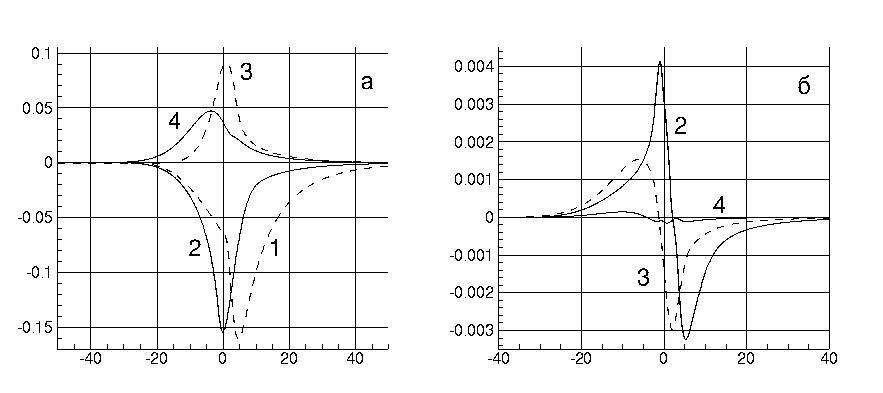
\includegraphics[width=1\linewidth]{U2D.png}}
\caption{Распределения вдоль трубы продольной (а) и радиальной (б) компоненты осесимметричной составляющей скорости $V_{2D}$ для нескольких расстояний от оси
трубы: 1–4 – r = 0, 0.4, 0.7, 0.9}
\label{U2D_pic}
\end{figure}

На фиг.~\ref{amp_pic} приведены распределения по $x$ среднеквадратичных по сечению трубы амплитуд трех составляющих движения: стационарной осесимметричной (отклонение от течения Пуазейля) $A_{2D}$, стационарной трехмерной $A_{3D}$ и колебательной $A_n$. Распределение $A_{2D}(x)$ соответствует фиг.~\ref{U2D_pic}. Отклонение от течения Пуазейля заметно на значительном отрезке от $x=-30$ до $x=40$. Максимум $A_{2D}$ составляет 8.4\%. Величина $A_{3D}$ характеризует интенсивность полосчатых структур. Как видно на фиг.~\ref{3D_img} полосчатые структуры появляются на некотором расстоянии вверх по потоку от головы порыва и сохраняются на значительном расстоянии позади него. В согласии с этим $A_{3D}(x)$ имеет выраженную асимметрию относительно точки $x=-2$, где эта величина достигает максимума. Интенсивность полос быстро падает вниз по потоку и сохраняется на значительном расстоянии в верхней части потока. В отличие от стационарных полосчатых структур, колебательная составляющая движения сосредоточена на сравнительно непротяженном отрезке трубы от $x=-5$ до $x=15$ с максимальной амплитудой в 4\% при $x=2.5$.

\begin{figure}[h]
\center{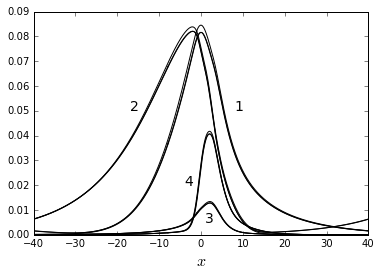
\includegraphics[width=0.5\linewidth]{amp.png}}
\caption{Распределения вдоль трубы среднеквадратичных по сечению амплитуд трех
составляющих движения: 1 – $V_{2D}$ (отклонение от течения Пуазейля); 2, 3 – продольная и поперечные компоненты скорости $V_{3D}$ ; 4 – $v_{n}$}
\label{amp_pic}
\end{figure}


В трехмерную стационарную составляющую движения $V_{x,3D}$ попадают полосы повышенной и пониженной скорости. Поле $V_{x,3D}$ в нескольких сечениях трубы изображено на рисунке~\ref{V3D_cs_pic}. В каждом сечении трубы полосы пониженной скорости ($V_{x,3D} < 0$) проходят через центр расчетной области, при $\theta = \pi/4$. Полосы повышенной скорости ($V_{x,3D} > 0$) попадают на границы расчетной области в угловом направлении, находящиеся при $\theta = 0, \pi/2$. Среднее поле скорости оказывается симметрично относительно плоскости, проходящей через центр расчетной области при $\theta = \pi/4$, так как поле скорости решения на сепаратрисе $\v$ имеет дополнительную симметрию отражения относительно указанной плоскости со сдвигом на половину периода по времени
\begin{equation}
\v(x, r, \pi/4 + \theta, t) = \v(x, r, \pi/4 - \theta, t + T/2). 
\end{equation} 


\begin{figure}[h]
\center{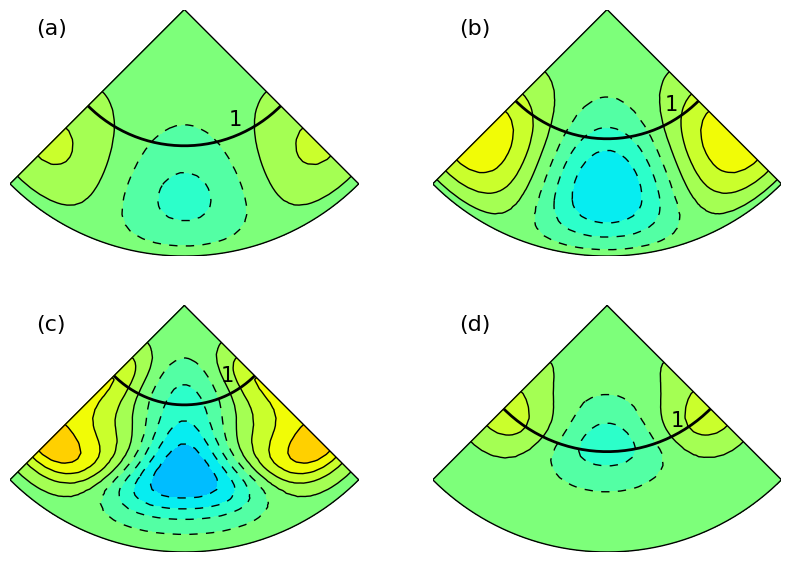
\includegraphics[width=0.8\linewidth]{V3D_cs.png}}
\caption{Распределения скорости полосчатых структур в нескольких сечениях трубы:
а–г --- x = –20, –10, 0, 5. Темный фон --- отрицательная скорость, светлый фон --- положительная скорость; 1 – линии нулевой скорости осесимметричной составляющей движения. В сечении (в) изображено векторное поле поперечного движения.}
\label{V3D_cs_pic}
\end{figure}

Пульсационная составляющая движения $\v_n$ представляет собой бегущую вниз по порыву волну. Чтобы это продемонстрировать, на рисунке~\ref{puls_ls_pic} изображено поле скорости $v_{x,n}$ в сечении $\theta = 0$ в четыре момент времени $t=0, T/4, T/2, 3T/4$, позволяющие представить изменение поля скорости на периоде изменения времени $T$. Хотя длина волны несколько меняется по мере продвижения вниз по трубе, её можно оценить $5R$, а скорость её перемещения вниз по потоку в $0.77U$, что на $0.08U$ выше скорости перемещения порыва вниз по трубе.  


\begin{figure}[h]
\center{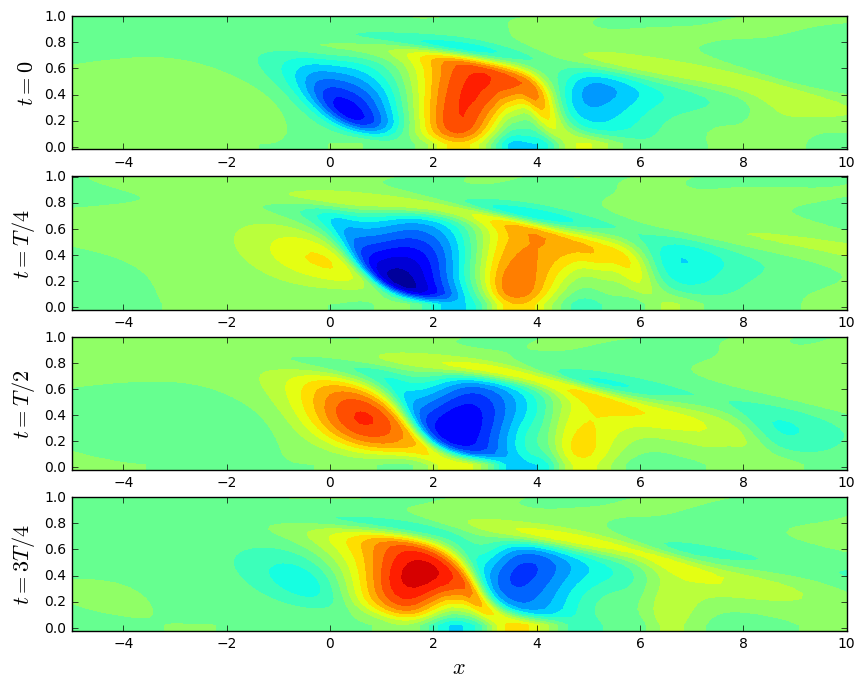
\includegraphics[width=0.8\linewidth]{v1_ls.png}}
\caption{Значение $v_{x,n}$ в сечении $\theta=0$ в моменты времени $0, T/4, T/2, 3T/4$. Синий --- отрицательное значение скорости, зеленый --- нулевое, красный --- положительное. Пульсационная составляющая движения перставляет собой бегущую вниз по потоку волну. }
\label{puls_ls_pic}
\end{figure}

\section{Механизм самоподдержания модельного порыва} 

Все описанные составляющие движения находятся в динамическом взаимодействии друг с другом. Как видно на рис.~\ref{amp_pic} наиболее локализованной вдоль трубы оказывается колебательная составляющая. Распределения среднеквадратичной амплитуды колебаний в нескольких сечениях трубы приведены на фиг.~\ref{puls_cs_pic}. Доминирующая мода колебательной составляющей пропорциональна $\exp(2\pi it/T)$ во времени и $\exp(2i\theta)$ в угловом направлении. Нелинейное взаимодействие колебательных мод порождает колебания на высших частотах, а также дает вклад в стационарную составляющую движения. В стационарной составляющей кроме осесимметричной части доминирует мода, пропорциональная $\exp(4i\theta)$, то есть с периодом $\pi/2$ в угловом направлении. Именно такой периодичности по углу соответствуют четыре пары полосчатых структур, наблюдающихся при решении задачи с условиями \eqref{sym_eq}, \eqref{per_eq}.

\begin{figure}[h]
\center{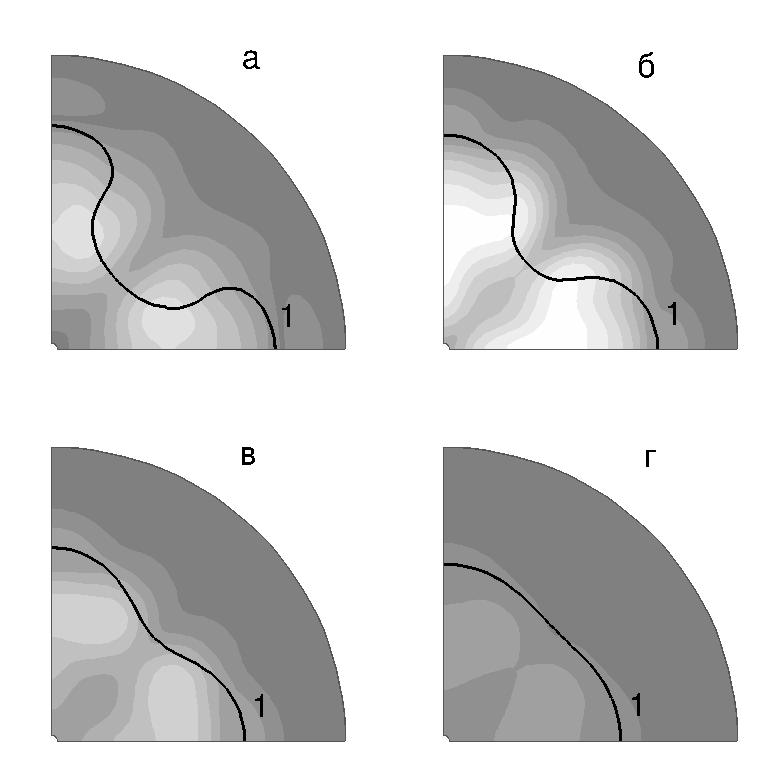
\includegraphics[width=0.8\linewidth]{puls_cs.png}}
\caption{Распределения среднеквадратичной амплитуды колебаний в нескольких сечениях трубы: а--г --- x = 0, 2.5, 5, 7.5. Максимальные значения выделены светлым
тоном. 1 – линия нулевой скорости относительного движения.}
\label{puls_ls_pic}
\end{figure}

Отметим, что непосредственный вклад колебаний в образование полос не велик. Основной механизм роста полос это так называемый лифтап (lift-up) эффект, связанный с появлением движения в перпендикулярной к основному потоку плоскости. Частицы жидкости, перемещающиеся от стенки в сторону оси трубы, приносят дефект скорости и образуют полосу замедления, а частицы двигающиеся в противоположном направлении --- от оси к стенке, образуют полосу ускорения. Основная роль колебательной составляющей в этом механизме состоит именно в порождении стационарного движения в поперечной плоскости, распределение среднеквадратичной амплитуды которого $A_\bot(x)$ также представлено на фиг.~\ref{amp_pic}. Как видно, область сосредоточения поперечного движения практически совпадает с областью существования колебаний. Некоторое уклонение $A_\bot(x)$ в заднюю сторону объясняется конвективным переносом этого движения (поперечное движение в основном возникает в периферийной части сечения трубы, где скорость потока в выбранной системе отсчета отрицательна).

Стационарное поперечное движение направлено от оси трубы к стенке в областях $\theta=k\pi/2$ и наоборот, от стенки к оси в промежуточных областях $\theta=\pi/4+k\pi/2$. Соответственно, в первых возникают полосы ускорения, во вторых --- замедления. Распределения скорости полосчатых структур в нескольких сечениях трубы приведены на фиг.~\ref{V3D_cs_pic}. В сечении $x=0$, где максимальна (среди сечений, представленных на фиг.~7) интенсивность поперечного движения, изображено также векторное поле поперечного движения, демонстрирующее лифт-ап механизм образования полосчатых структур. На всех сечениях фиг.~\ref{V3D_cs_pic} сплошной линией изображена линия нулевой скорости осесимметричной составляющей движения в подвижной системе отсчета. В приосевой области, ограниченной этой линией, скорость положительна, а в периферийной --- отрицательна. Как видно из рисунков, полосчатые структуры во всех сечениях кроме самого переднего из представленных ($x=5$) располагаются в области отрицательной относительной скорости. Осесимметричное движение с отрицательной скоростью переносит полосчатые структуры в заднюю часть порыва, где они формируют картину, похожую на вытянутые щупальца медузы (см. фиг.~\ref{3D_img}). При $x>5$ полосчатые структуры концентрируются в приосевой части трубы и конвектируются вперед положительной скоростью относительного движения, благодаря чему в передней части порыва $A_{3D}$ сохраняет заметную величину, несмотря на отсутствие поперечного движения.


\section{Линейная устойчивость стационарного течения}

Полосчатые структуры достигают максимальной своей амплитуды в области $x\in[-5,0]$, где создаются условия для возникновения колебаний. Наиболее вероятный механизм генерации колебаний --- механизм потери устойчивости стационарной составляющей течения. Для проверки этой гипотезы стационарное течение с полем скорости $\V$ было исследовано на устойчивость к малым возмущениям. Линеаризованные относительно возмущений уравнения с некоторыми случайными начальными условиями интегрировались по времени до выхода решения на режим экспоненциального изменения. Обнаружено, что действительно поле скорости $\V$ неустойчиво к малым возмущениям. Растущее возмущение $\sim\exp(\lambda+i\omega)t$ имеет коэффициент роста $\lambda=0.012$ и частоту $\omega=0.116$, близкую к частоте колебаний $2\pi/60=0.105$ в решении на сепаратрисе. Что еще более существенно, распределение амплитуды колебаний в растущем решении задачи линейной устойчивости оказывается близким к соответствующим распределениям колебательной составляющей решения на сепаратрисе. Таким образом, нет сомнений, что механизмом появления колебаний является линейная неустойчивость стационарной составляющей движения.

Отметим, что неустойчивость полосчатых структур является неотъемлемой составляющей всех сценариев самоподдержания турбулентности в пристенных течениях. При этом чаще всего предполагается, что неустойчивость возникает в пристенных областях полос замедленного движения, где в локальном профиле скорости $U(r)$ на фоне наибольшего градиента появляется точка перегиба --- источник неустойчивости в механизме типа Кельвина--Гельмгольца. В частности, именно такой механизм предлагается в качестве механизма возникновения колебаний в турбулентном порыве в \cite{Shumizu2009}. В рассматриваемом нами решении на сепаратрисе это определенно не так. Как видно на фиг.~6 в сечении $x=0$, соответствующем максимальной скорости роста колебаний, амплитуда колебаний минимальна как раз в области полосы замедления ($\theta=\pi/4$). Наибольшие колебания развиваются наоборот вблизи полос ускорения, а если быть более точным, в промежуточных областях между полосами. В этих областях стационарная составляющая скорости течения претерпевает наибольшее изменение и имеет точки перегиба, но не как функция радиальной переменной, а как функция угла. Во всех сечениях фиг.~\ref{puls_cs_pic} сплошными линиями изображены линии нулевой относительной скорости стационарной составляющей течения. Видно, что в сечении $x=0$, где происходит основной рост колебаний, в областях максимальной амплитуды колебаний наблюдается наиболее быстрое изменение скорости как функции угловой переменной.

Отметим также, что точки максимального роста колебаний находятся на линии $r\approx0.4$, что соответствует нулевой относительной скорости. По этой причине область порождения колебаний остается неподвижной относительно порыва. Интересно, что в этой же области ($x=0,\ r\approx0.4$) происходит смена знака радиальной компоненты осесимметричной составляющей скорости (см. фиг.~4,б). При $x<0$ радиальная скорость положительна, поэтому колебания, возникшие в задней части порыва, относятся в сторону стенки трубы, где относительная скорость отрицательна, и уносятся в хвостовую часть порыва. Наоборот, при $x>0$ радиальная скорость направлена к оси трубы, туда же, в область положительной скорости, сносятся и колебания, обнаруживающиеся в передней части порыва.

Целесообразно проверить на линейную устойчивость однородное вдоль трубы поле скорости. 


\section{Бегущая волна}

Как было показано в предыдущем разделе, в основе механизма самоподдержания решения на сепаратрисе лежит бегущая вниз по порыву волна. Оказывается возможным получить аналогичную волну в более простой форме. Длину волны, возникающей в модельном порыве, можно оценить в $5R$. Если применить метод поиска решения на сепаратрисе к расчетной области длиной $L_x = 5R$, то решение на сепаратрисе выходит на режим бегущей волны, двигающейся в низ по течению. В подвижной системе отсчета решение оказывается стационарным, что делает его еще более доступным для исследования, чем модельный порыв. Исследование этой бегущей волны показало, что она качественно воспроизводит многие особенности модельного порыва, а также позволило установить новые детали механизма самоподдержания, связанные с образование продольных вихрей. Применимость полученных при исследовании бегущей волны результатов к модельному порыву позже будет продемонстрированная отдельно. 


Бегущая волна была найдена также при $\Re = 2200$, скорость её сноса оказалась равна $c_f = $

Как и при исследовании модельного порыва, разделим поле скорости бегущей волны на стационарную и пульсационную составляющею. Осреднеие по времени в случаемоедльного порыва проводилось в системе отсчета, связанной с порывом, в которой бегущая волна, бегущая вниз по порыву волна оказывалась подвижной. 

\section{Механизм образования продольных вихрей.}

Продольные вихри в стационарной составляющей движения возникают в результате нелинейного взаимодействия пульсаций. Это, в частности, подтверждается фактом совпадения областей концентрации продольных вихрей и пульсаций вдоль трубы. Прояснить процесс формирования продольных вихрей позволяет анализ уравнения, описывающего эволюцию продольной завихренности, полученного применением оператора Ротора к уравнению Навье-Стокса \eqref{NSeq_cf}:
\begin{equation}\label{ox_eq}
\pd{\omega_x}{t} - \nu\nabla^2 \omega_x =  -  (\v - \c_f, \nabla) \omega_x + (\om, \nabla) v_x
\end{equation}
Здесь $\om = (\omega_x, \omega_r, \omega_\theta) = \rot \v$ --- вектор завихренности, $\c_f$ --- скорость перемещения системы отсчета. Уравнение для стационарной составляющей продольной завихренности получается после осреднения \eqref{ox_eq} по времени в системе отсчета, связанной с порывом:
\begin{equation}\label{OX_eq}
\pd{\Omega_x}{t} - \nu\nabla^2 \Omega_x = - (\V - \c_f, \nabla) \Omega_x + (\Om, \nabla) V_x - \overline{(\v', \nabla) \omega'_x}^t + \overline{ (\om', \nabla) v'_x }^t
\end{equation}
Здесь  $\Om=(\Omega_x, \Omega_r, \Omega_\theta)$ и $\om'=(\omega'_x, \omega'_r, \omega'_\theta)$ средняя и пульсационная составляющие вектора завихренности. Черта над выражением --- знак осреднения по переменной, указанной верхним индексом. В правой части \eqref{OX_eq} первая пара членов описывает изменение продольной завихренности за счет конвективного переноса и деформации вихревых линий осредненного течения, а вторая пара выражает порождение средней завихренности пульсационным движением. При отсутствии пульсаций продольная завихренность постепенно исчезает под действием вязкости. В рассматриваемом течении система находится в равновесии и стационарная продольная завихренность во времени не меняется. Вязкие диссипация и диффузия компенсируются генерацией завихренности членами в правой части \eqref{OX_eq}.

Для выявления определяющих механизмов генерации средней продольной завихренности удобнее рассмотреть уравнение эволюции квадрата $\Omega_x$, получающееся домножением всех членов \eqref{OX_eq} на $2\Omega_x$. Положительный или отрицательный знак у полученных таким образом выражений в правой части уравнения показывает соответственно положительный или отрицательный вклад этого члена в изменение $\Omega_x^2$, а, следовательно, и в интенсивности поперечного движения. Распределение $\Omega_x^2$ по сечению трубы представлено на рис.~\ref{OXgen_pic}(a). В большей части сечения трубы средняя продольная завихренность близка к нулю. Область концентрации $\Omega_x$ расположена между полосами повышенной и пониженной скорости вблизи области максимальной амплитуды пульсаций.

\begin{figure}[h]
\center{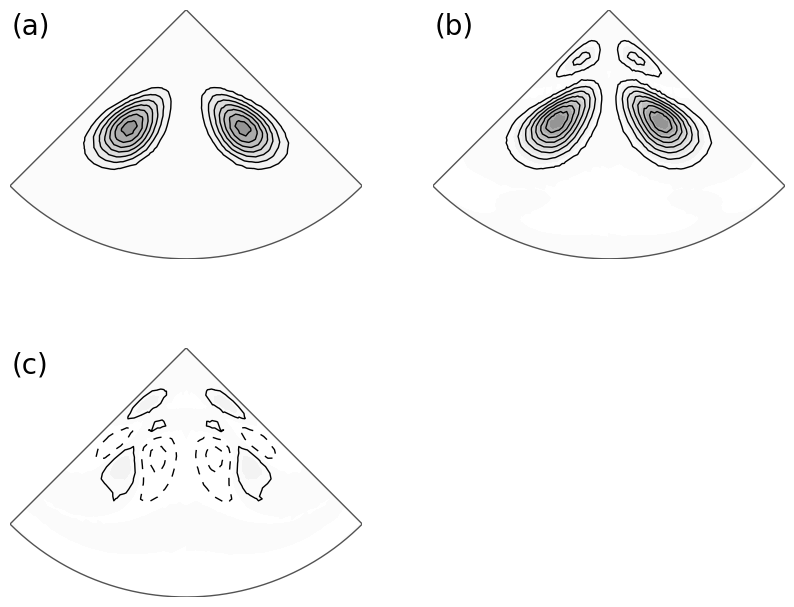
\includegraphics[width=0.9\linewidth]{OXgen.png}}
\caption{Распределение по сечению трубы $\Omega_x^2$ --- (a), вклад в производство $\Omega_x^2$ слагаемых, соответствующих выделенным в \eqref{OXgen_terms} --- (b), вклад остальных слагаемых в правой части \eqref{OX_eq} --- (с). Сплошные линии соответствуют положительным значениям, прерывистые --- отрицательным.}
\label{OXgen_pic}
\end{figure}

При анализе уравнения \eqref{OX_eq} обнаружено, что два слагаемых в правой части, а именно
\begin{equation}\label{OXgen_terms}
 - \overline{v'_x \frac{\d \omega'_x}{\d x}} + \overline{ \omega'_x \frac{\d v'_x}{\d x} },
\end{equation}
вносят определяющий вклад в производство средней продольной завихренности. Соответствующее сумме \eqref{OXgen_terms}  распределение в уравнении для $\Omega_x^2$ представлено на рис.~\ref{OXgen_pic}(b), а вклад остальных слагаемых правой части \eqref{OX_eq} показан на рис.~\ref{OXgen_pic}(c). Распределение генерации $\Omega_x^2$ выделенными в \eqref{OXgen_terms} членами практически совпадает по форме с распределением $\Omega_x^2$, тогда как вклад остальных членов не имеет выраженного распределения и более чем на порядок уступает по суммарному вкладу в генерацию $\Omega_x^2$. Таким образом, нет сомнения в том, что стационарные продольные вихри возникают в основном за счет действия выделенной в \eqref{OXgen_terms} пары слагаемых.

Отметим, что пульсации, соответствующие старшей собственной функции линейной задачи об устойчивости среднего стационарного течения, также демонстрируют приведенный выше механизм образования стационарных продольных вихрей. Важно, что это наблюдается только в том случае, когда при анализе устойчивости учитываются как продольная, так и поперечная составляющие среднего течения. Принято считать, что поперечное движение, определяя угловую неоднородность в распределении продольной скорости среднего течения, не может существенным образом влиять на свойства его устойчивости вследствие незначительности своей амплитуды. Поэтому при исследовании линейной устойчивости подобных течений, например, полосчатых структур в турбулентных потоках, наличие поперечного движения обычно не принимается во внимание. В нашем случае пренебрежение поперечным движением приводит к тому, что стационарное течение оказывается линейно устойчивым. Что еще более важно, наименее затухающее возмущение не воспроизводит при этом описанный механизм формирования продольных вихрей. Это связанно с тем, что форма пульсаций продольной завихренности $\omega'_x$ качественно меняется, хотя пульсации продольной скорости $v'_x$ сохраняют свою форму практически неизменной. Тем самым нарушается согласованность  $v'_x$ и $\omega'_x$, необходимая для обеспечения нужного вклада выражения \eqref{OXgen_terms} в производство продольной завихренности.

Каждое из двух слагаемых в \eqref{OXgen_terms} дает примерно половину общего вклада в производство средней продольной завихренности. Это значит, в частности, что колебания $\d v'_x/\d x$ и $\omega'_x$ положительно коррелированы в области концентрации положительной $\Omega_x$ и отрицательно коррелированы в области концентрации отрицательной $\Omega_x$. То же относится и к колебаниям $-v'_x$ и $\d \omega'_x/\d x$. Расчет соответствующих коэффициентов корреляции показывает, что они близки к $\pm1$ в соответствующих областях. 


\section{Механизм возникновения пульсаций продольной завихренности}

Для выявления механизма формирования такой связи между пульсациями продольных компонент скорости и завихренности рассмотрим уравнение эволюции $\omega'_x$, получающееся вычитанием \eqref{OX_eq} из \eqref{ox_eq}:
\begin{multline}\label{ox1_eq}
\pd{\omega'_x}{t} - \nu \nabla^2 \omega'_x = - (\V - \c, \nabla) \omega'_x - (\v', \nabla) \Omega_x
+(\Om, \nabla) v'_x + (\om', \nabla) V_x -\\- (\v', \nabla) \omega'_x  + (\om', \nabla) v'_x  + \overline{(\v', \nabla) \omega'_x)}  - \overline{(\om', \nabla)}
\end{multline}
Работать удобнее с уравнением, описывающим изменение среднего квадрата пульсаций продольной завихренности $\overline{\omega'^2_x}$, получающимся умножением на $2\omega'_x$ каждого из слагаемых в \eqref{ox1_eq} и последующим осреднением по времени. Как и раньше, осреднение по времени производится в подвижной системе отсчета. Слагаемые в этом уравнении не зависят от времени, сумма слагаемых в правой части балансируется вязким членом в левой части. Как и в предыдущем случае, среди всех слагаемых правой части удается выделить существенные, ответственные за возникновение пульсаций $\omega'_x$.


Распределение $\overline{\omega'^2_x}$ по сечению трубы с максимальным уровнем пульсаций изображено на рис.~\ref{ox1gen_pic}(a). Основные пульсации $\omega'_x$ наблюдаются в центре расчетной области около оси трубы. На месте расположения продольных вихрей также присутствуют пульсации $\omega'_x$, но меньшей интенсивности. В остальной части трубы их амплитуда близка к нулю. Обнаружено, что за генерацию пульсаций $\omega'_x$ в центральной части трубы и на месте продольных вихрей отвечают два разных механизма. Первый дает пульсации большей амплитуды, однако, за возникновение стационарных продольных вихрей ответственны пульсации, производимые вторым механизмом, так как именно они оказываются согласованными с пульсациями $v'_x$ нужным образом.


\begin{figure}[h]
\center{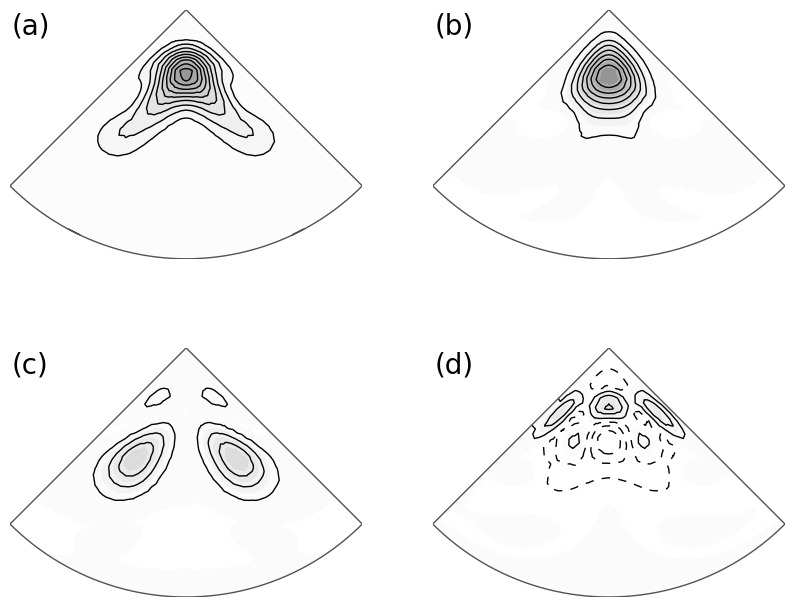
\includegraphics[width=0.9\linewidth]{ox1gen.png}}
\caption{Распределение среднего квадрата пульсаций продольной завихренности --- а, вклад в производство $\left<\omega'^2_x \right>$ слагаемых \eqref{ox1gen_add_terms} --- (b), слагаемого \eqref{ox1gen_main_terms} --- (c) и суммы остальных слагаемых правой части \eqref{ox1_eq} --- (d).}
\label{ox1gen_pic}
\end{figure}


Первый механизм формирования $\omega'_x$ связан с наличием нормальных к стенке вихрей в пульсационной составляющей движения. Можно провести аналогию между неустойчивостью, возникающей на полосе замедления, и неустойчивостью в следе за телом. Пульсационная составляющая движения напоминает дорожку Кармана. В ней можно выделить последовательность нормальных к стенке вихрей чередующегося знака, двигающихся вниз по полосе пониженной скорости. Им соответствуют области повышенной амплитуды пульсаций радиальной завихренности $\omega'_r$. Между полосой замедления и осью трубы имеется значительный радиальный градиент продольной скорости $\d V_x/ \d r$. В его присутствии нормальные к стенке вихри поворачиваются так, что приобретают продольную составляющую $\omega'_x$. Кроме того, наличие радиального градиента $\d V_x/ \d r$ связано с наличием угловой завихренности $\Omega_\theta = \d V_r / \d x - \d V_x / \d r$. Радиальная пульсационная завихренность $\omega'_r = \d v'_x / r \d \theta - \d v'_\theta / \d x$ за счет первого из слагаемых поворачивает стационарные угловые вихри так, что те также приобретают пульсационную продольную составляющую. В уравнении \eqref{ox1_eq} за описанный механизм отвечают слагаемые:
\begin{equation}\label{ox1gen_add_terms}
\frac{\d \omega'_x}{\d t} = \omega'_r \frac {\d V_x}{\d r} +
\frac{\Omega_\theta}{r} \frac{\d v'_x}{\d \theta} + ...
\end{equation}
Несмотря на то, что выделенные в \eqref{ox1gen_add_terms} слагаемые имеют противоположные знаки и в значительной степени компенсируют друг друга при сложении, их вклад в производство $\omega'_x$ значителен (см. рис.~\ref{ox1gen_pic}(b)). Они определяют форму пульсаций $\omega'_x$ в области между полосой замедления и осью трубы, где пульсации $\omega'_x$ достигают наибольшего значения. Эти пульсации, однако, практически не участвуют в образовании стационарной составляющей продольной завихренности. Это объясняется тем, что колебания $\omega'_x$, рождающиеся в результате описанного механизма, близки по фазе к колебаниям $v'_x$, так что сомножители каждого из слагаемых в выражении \eqref{OXgen_terms} оказываются в противофазе и при осреднении дают близкие к нулю значения.


Второй механизм образования пульсаций продольной завихренности $\omega'_x$ связан с перераспределением уже существующей стационарной продольной завихренности $\Omega_x$ за счет пульсационной составляющей продольной скорости $v'_x$ (эффект сжатия/растяжения вихревых линий). В уравнении \eqref{ox1_eq} за описываемый механизм отвечает слагаемое
\begin{equation}\label{ox1gen_main_terms}
\frac{\d \omega'_x}{\d t} = \Omega_x \frac {\d v'_x}{\d x} + ...
\end{equation}
Выделенное в \eqref{ox1gen_main_terms} слагаемое стремится произвести пульсации $\omega'_x$, пропорциональные $\d v'_x / \d x$, что обеспечивает наибольшую эффективность образования $\Omega_x$ посредством их нелинейного взаимодействия. Важно, что коэффициентом пропорциональности в \eqref{ox1gen_main_terms} выступает значение средней продольной завихренности, таким образом, механизм включается именно в областях концентрации $\Omega_x$. При этом производимые пульсации $\omega'_x$ положительно пропорциональны пульсациям  $\d v'_x / \d x$ при $\Omega_x>0$ и отрицательно пропорциональны при $\Omega_x<0$, что обеспечивает максимально возможную эффективность производства средней продольной завихренности нужного знака посредством второго из слагаемых выражения \eqref{OXgen_terms}. Очевидно, что пульсации $-v'_x$ и $\d \omega'_x / \d x$ в этом случае также согласованы нужным образом, так что первое слагаемое \eqref{OXgen_terms} близко по значению ко второму.


На рис.~\ref{ox1gen_pic}(c) приведен вклад выделенного в \eqref{ox1gen_main_terms} слагаемого в производство $\overline{\omega'^2_x}$. Нет сомнения, что именно это слагаемое определяет форму пульсаций в области существования продольных вихрей между полосами повышенной и пониженной скорости. Суммарный вклад других слагаемых правой части \eqref{ox1_eq}, не попавших на рис.~\ref{ox1gen_pic}(b,c), изображен на рис.~\ref{ox1gen_pic}(d). Эти слагаемые не имеют существенного значения в процессе генерации $\omega'_x$, их суммарный вклад не превышает нескольких процентов.

Описанный механизм генерации пульсаций продольной завихренности проявляется в области, где фазовая скорость волны, соответствующей пульсационной составляющей течения, близка по значению к локальной продольной скорости среднего течения. На удалении от точки генерации пульсаций, где фазовая скорость волны существенно отличается от средней скорости, выделенный в \eqref{ox1gen_main_terms} механизм генерации $\omega'_x$ практически не работает. Это объясняется тем, что в системе отсчета, связанной с волной, образующаяся посредством механизма \eqref{ox1gen_main_terms} $\omega'_x$ сносится вдоль трубы средним течением. При этом теряется согласованность фаз между $\d v'_x / \d x$ и $\omega'_x$, что делает её рост невозможным.


Описанный механизм генерации пульсаций продольной завихренности объясняет необходимость учета поперечного движения при исследовании устойчивости стационарного течения. Пренебрежение связанной с поперечным движением $\Omega_x$ делает невозможным генерацию $\omega'_x$ в форме, необходимой для сохранения поперечного движения, а следовательно и всего процесса самоподдержания пульсаций.

